\begin{frame}{Few-shot Prompts}
  \vspace{-0.3em}
  \begin{itemize}
    \item Few-shot prompting allows us to provide \textbf{exemplars in prompts} to steer the model towards better performance
  \end{itemize}
  \vspace{0.3em}
  \begin{center}
    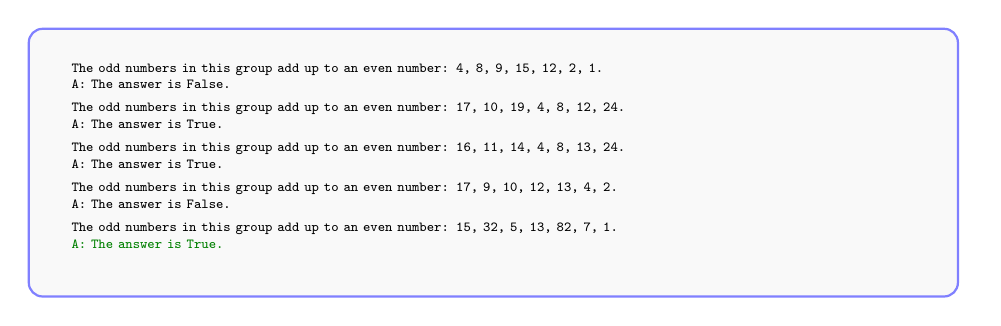
\begin{tikzpicture}
      % Outer rounded rectangle with blue border
      \node[draw=blue!50, thick, rounded corners=5pt, fill=gray!5, minimum width=11.8cm, minimum height=3.4cm, anchor=north west, inner sep=0pt] (fsbox) at (0,2.7) {};

      % Main multi-line code block in gray font, monospaced
      \node[anchor=north west, font=\ttfamily\tiny, text width=11.2cm, align=left, inner sep=2.5mm] at ([xshift=0.3cm, yshift=-0.20cm]fsbox.north west) {%
The odd numbers in this group add up to an even number: 4, 8, 9, 15, 12, 2, 1.\\
A: The answer is False.\\[0.45em]
The odd numbers in this group add up to an even number: 17, 10, 19, 4, 8, 12, 24.\\
A: The answer is True.\\[0.45em]
The odd numbers in this group add up to an even number: 16, 11, 14, 4, 8, 13, 24.\\
A: The answer is True.\\[0.45em]
The odd numbers in this group add up to an even number: 17, 9, 10, 12, 13, 4, 2.\\
A: The answer is False.\\[0.45em]
The odd numbers in this group add up to an even number: 15, 32, 5, 13, 82, 7, 1.\\
\textcolor{green!50!black}{A: The answer is True.}
      };
    \end{tikzpicture}
  \end{center}
  \vspace{-0.2em}
  {\footnotesize
    \textbf{The last answer is wrong:} the odd numbers are 15, 5, 13, 7, 1, which sum to 41, an odd
    number, so the answer is False. Exemplars alone do not teach the model to carry out the
    intermediate arithmetic.
  }
\end{frame}
